% Glossar
%\setglossarysection{section}
%\glsaddall
\setglossarysection{chapter}
\printglossary[numberedsection,style=altlist,title=Begriffsdefinitionen]
\label{chap:Definitionen}

%ANFORDERUNGSANALYSE
\includepdf[pages=2, scale=0.7, delta=0cm -2cm, pagecommand=\chapter{Auszug Fragestellungen Anforderungsanalyse}\label{att:anforderung}, offset=0 -2cm]{attachments/Anforderungsanalyse.pdf}
\includepdf[pages=3-7, scale=0.9, offset=0 -0.6cm, pagecommand=\thispagestyle{headings}]{attachments/Anforderungsanalyse.pdf}
\newpage


%PERSONAS
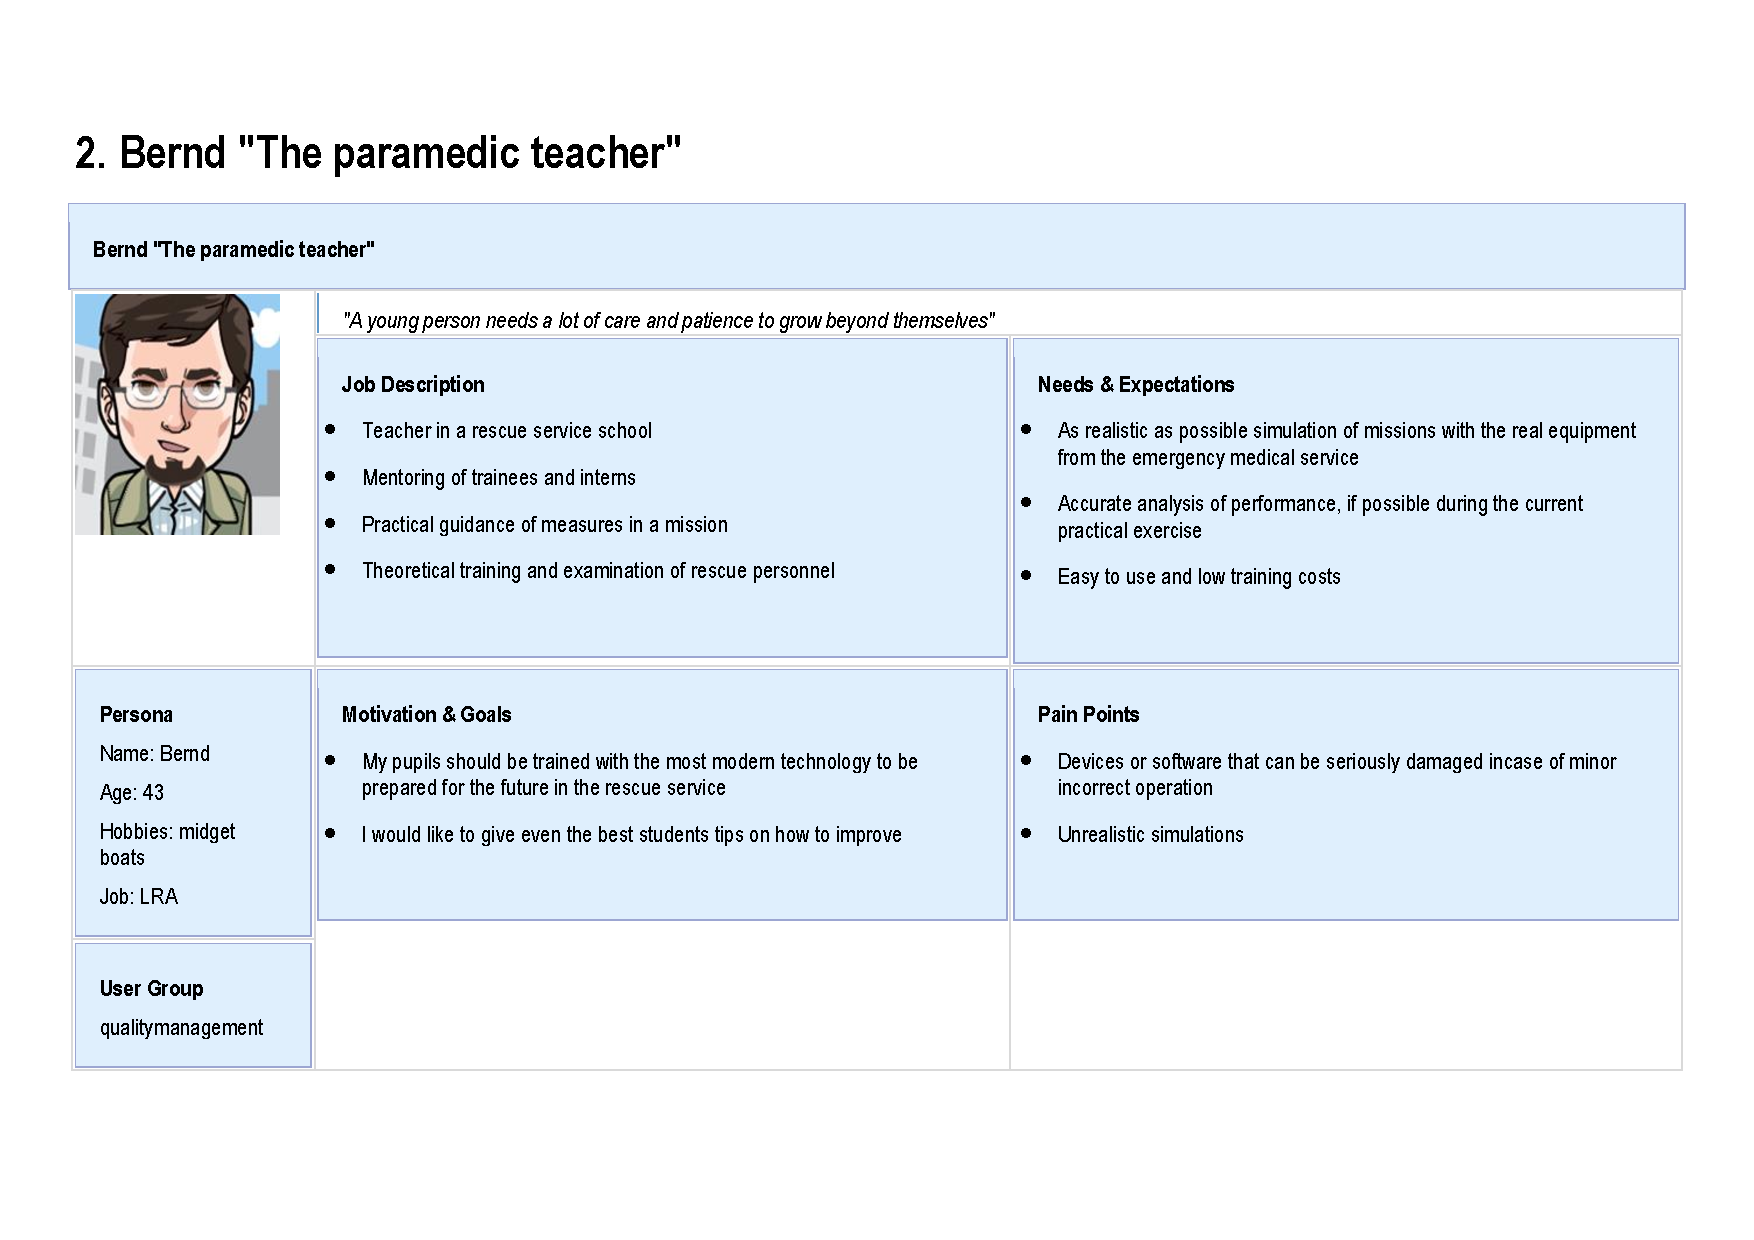
\includepdf[pages=1-2, nup=1x2, scale=0.9, delta=0cm -2cm, pagecommand=\section{Personas}\label{att:personas}, offset=0 -0.9cm]{attachments/Personas.pdf}

\includepdf[pages=3-4, nup=1x2, scale=0.9, delta=0cm -1cm, pagecommand=\thispagestyle{headings}]{attachments/Personas.pdf}


%EVALUATION
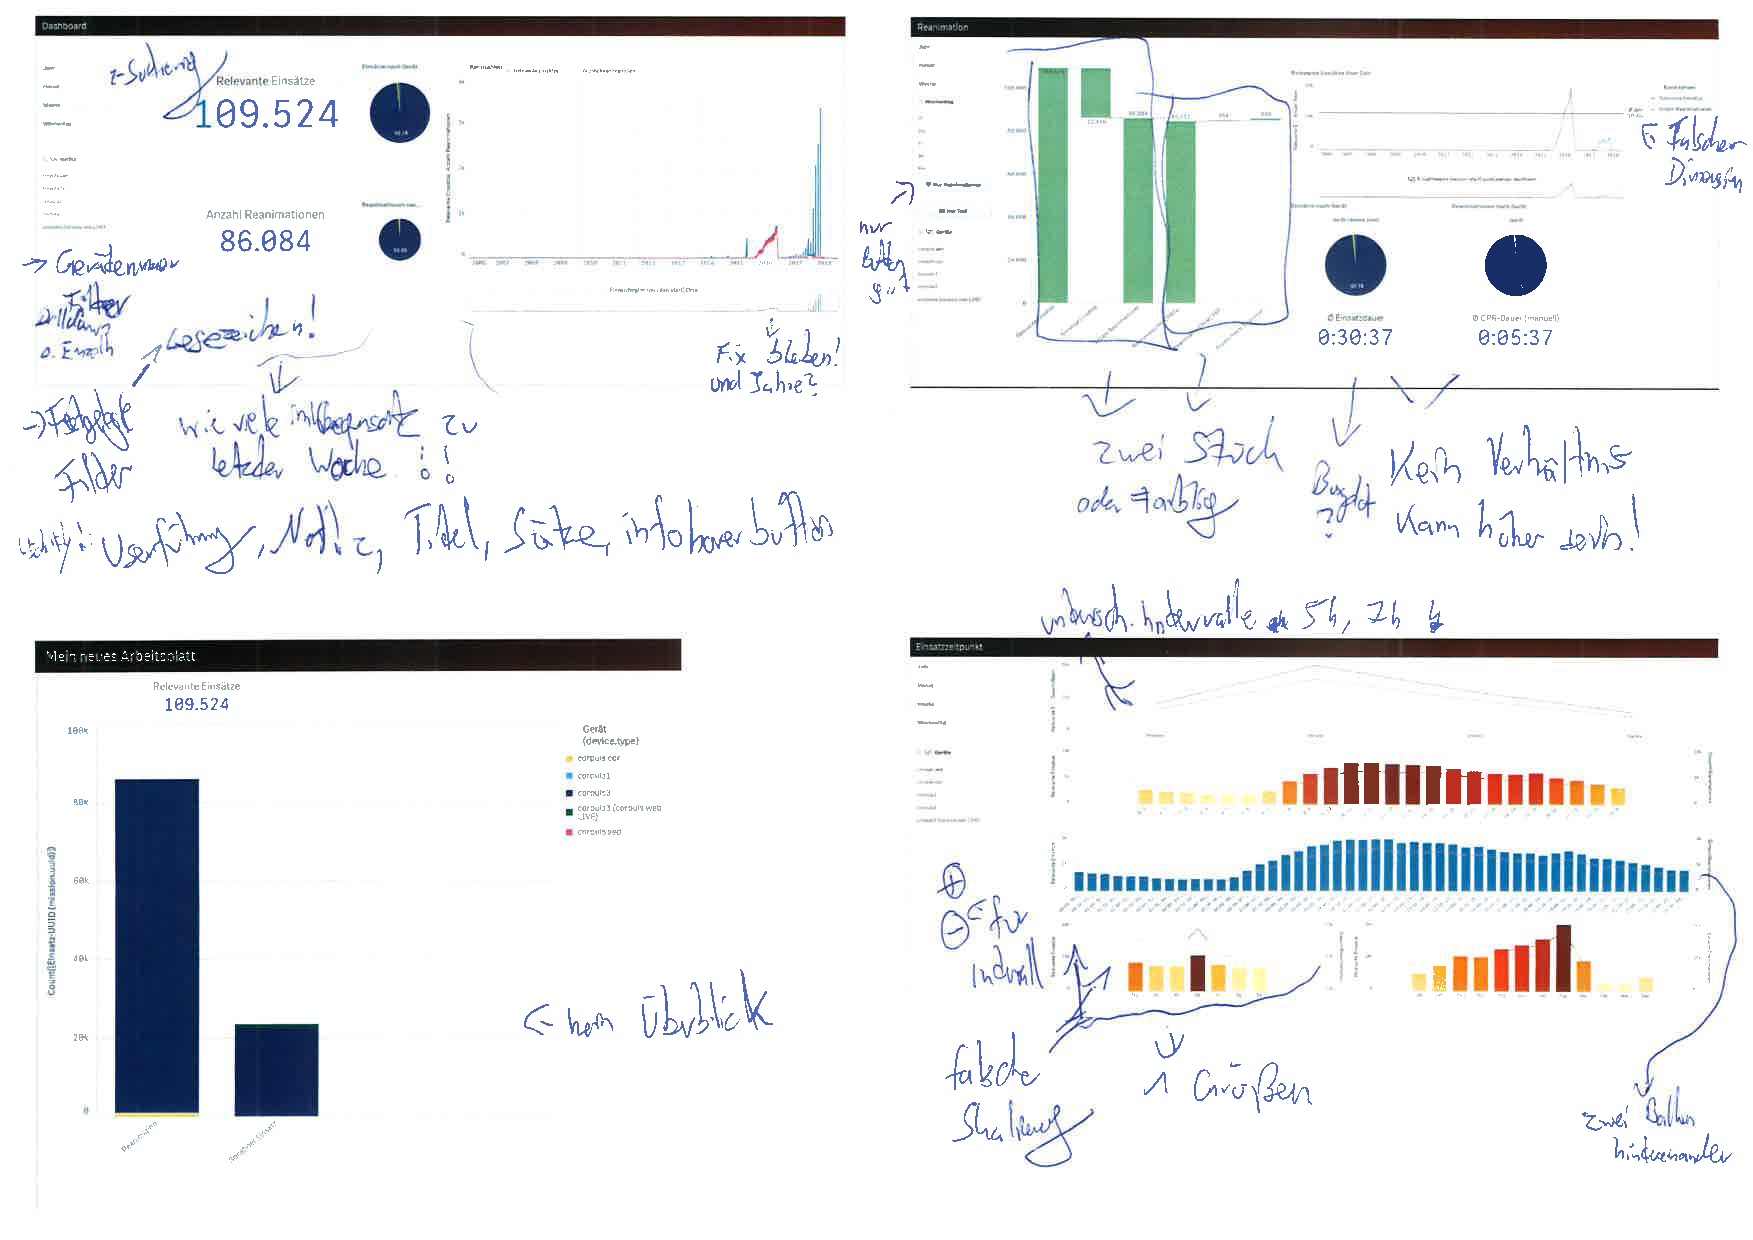
\includepdf[pages=1-2, nup=1x2, scale=0.7, pagecommand=\chapter{Evaluation}\label{att:evaluation}, offset=0 -2cm]{attachments/ALL_EVALUATION2.pdf}
%\includepdf[pages=3, nup=1x2, scale=0.7]{attachments/ALL_EVALUATION2.pdf}
\includepdf[pages=4-15, nup=2x2, scale=0.8,  pagecommand=\thispagestyle{headings}]{attachments/ALL_EVALUATION2.pdf}
\includepdf[pages={3, 16-22}, nup=1x2, scale=0.8, pagecommand=\thispagestyle{headings}]{attachments/ALL_EVALUATION2.pdf}

%\chapter{Dashboards}
%\includepdf[pages=-, nup=1x2, scale=0.6, landscape=true]{attachments/d12.pdf}


%DASHBOARDS
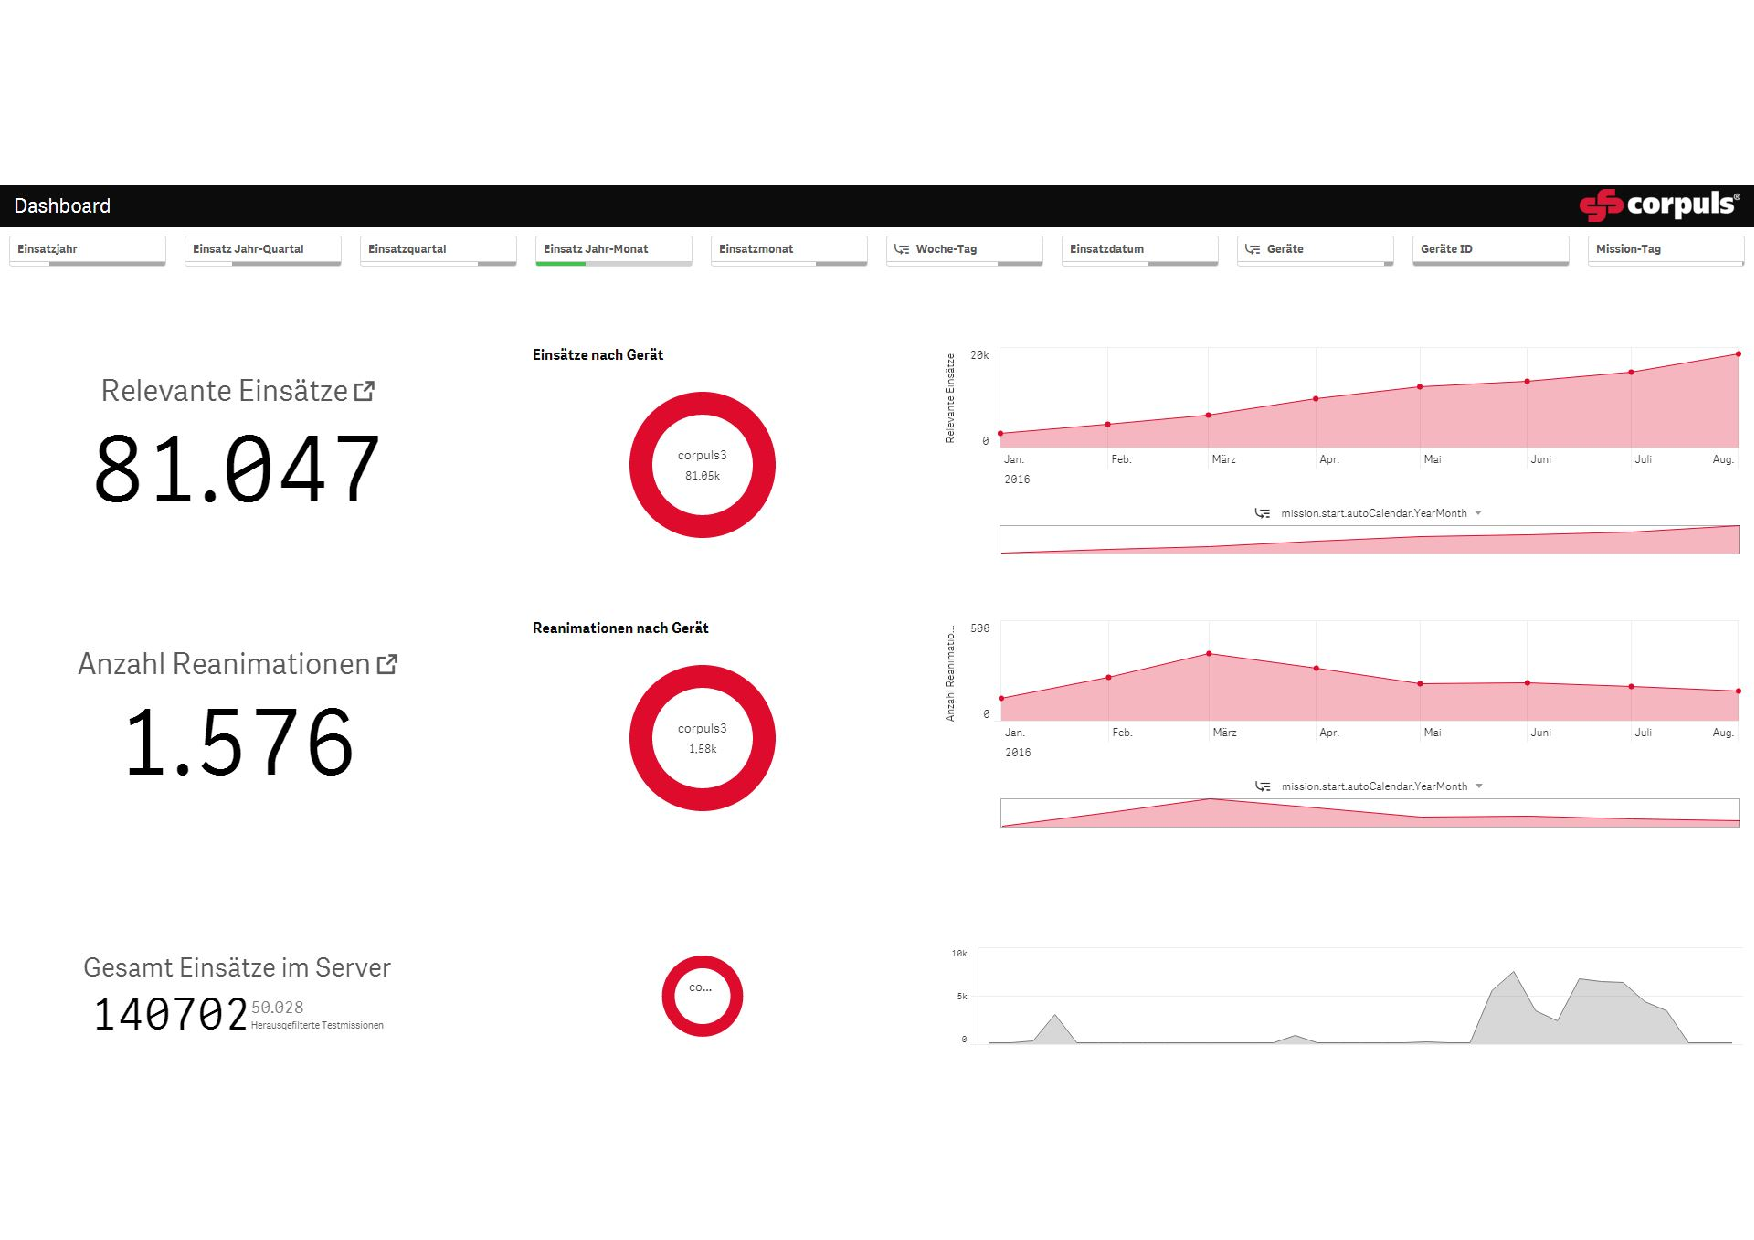
\includepdf[pages=1-2, nup=1x2, scale=0.7, pagecommand=\chapter{Dashboards}\label{att:dashboards}, offset=0 -2cm]{attachments/dashboards.pdf}

\includepdf[pages=3-19, nup=1x2, scale=0.83, pagecommand=\thispagestyle{headings}]{attachments/dashboards.pdf}

%\chapter{JSON Custom Theme}
